\documentclass[a4paper, 12pt]{article}
\usepackage[utf8x]{inputenc}
\usepackage{cmap}
\usepackage[english, russian]{babel}
\usepackage{indentfirst}
\usepackage[left=20mm, top=20mm, right=20mm, bottom=20mm]{geometry}
\usepackage{tikz}
\usepackage{float}
\usepackage{amsmath, amsfonts, amssymb}
\usepackage{graphicx}
\usepackage{fancybox, fancyhdr}
\usepackage{hyperref}
\usepackage{listings}
\usepackage{caption}
\usepackage{subcaption}
\usepackage{xcolor}
\pagestyle{fancy}
\fancyhf{}
\fancyhead[L]{Лабораторная работа №5}
\fancyhead[R]{Частотные методы}
\fancyfoot[C]{\thepage}
\graphicspath{{images/}}
\usetikzlibrary{patterns}
\definecolor{LightGray}{gray}{0.95}
\definecolor{LightGray2}{gray}{0.7}
\lstdefinestyle{code}{
    language=Python,
    basicstyle=\footnotesize\ttfamily,
    numbers=left,
    numberstyle=\scriptsize\color{gray},
    stepnumber=1,
    numbersep=5pt,
    backgroundcolor=\color{LightGray},
    showspaces=false,
    showstringspaces=false,
    showtabs=false,
    tabsize=4,
    captionpos=b,
    breaklines=true,
    breakatwhitespace=false,
    frame=single,
    rulecolor=\color{LightGray2},
    linewidth=\linewidth,
    keywordstyle=\color{blue}\bfseries,
    commentstyle=\color{green!40!black},
    stringstyle=\color{purple},
    escapeinside={\%*}{*)},
    inputencoding=utf8x,
    xleftmargin=0pt,
    framexleftmargin=0pt,
    framexrightmargin=0pt
}
\lstset{style=code}
\hypersetup{
    colorlinks=true,
    linkcolor=blue,
    filecolor=magenta,
    urlcolor=cyan,
    pdftitle={contents setup},
    pdfpagemode=FullScreen,
}
\setlength{\parskip}{1.5mm}
\setlength{\headheight}{15pt}
\setlength{\footskip}{15pt}
\allowdisplaybreaks
\DeclareMathOperator{\sinc}{sinc}
\newcommand{\frc}[2]{\raisebox{2pt}{$#1$}\big/\raisebox{-3pt}{$#2$}}

\begin{document}
    \begin{titlepage}

        \begin{center}
        
\includegraphics[width=0.3\textwidth]{itmo.png} % requires itmo.png in /images folder
        \vfill

        Федеральное государственное автономное образовательное учреждение высшего образования
        «Национальный Исследовательский Университет ИТМО»\\

        \vfill
        {\large\bf ЛАБОРАТОРНАЯ РАБОТА №5}\\
        {\large\bf ПРЕДМЕТ «ЧАСТОТНЫЕ МЕТОДЫ»}\\
        {\large\bf ТЕМА «СВЯЗЬ НЕПРЕРЫВНОГО И ДИСКРЕТНОГО»}
        \vfill

        \begin{flushright}
            \begin{minipage}{.45\textwidth}
            {
                \hbox{Лектор: Перегудин А. А.}
                \hbox{Практик: Пашенко А. В.}
                \hbox{Студент: Румянцев А. А.}
                \hbox{Поток: ЧАСТ.МЕТ. 1.3}
                \hbox{}
                \hbox{Факультет: СУиР}
                \hbox{Группа: R3241}
            }
            \end{minipage}
        \end{flushright}

        \vfill

        Санкт-Петербург\\
        2024
        \end{center}
    \end{titlepage}

    \tableofcontents

    \newpage
    \section{Задание 1. Непрерывное и дискретное преобразование Фурье}
    Рассмотрим прямоугольную функцию $\Pi:\mathbb{R}\rightarrow\mathbb{R}$:
    $$\Pi(t)=
    \begin{cases}
        1, & |t| \leq \frc{1}{2},\\
        0, & |t| > \frc{1}{2}.
    \end{cases}$$


    \subsection{Истинный Фурье-образ}
    Найдем аналитическое выражение для Фурье-образа прямоугольной функции
    $$\hat{\Pi}(\nu)=\int\limits_{-\infty}^{+\infty}\Pi(t)e^{-2\pi i \nu t}\,dt=\int\limits_{-\frac{1}{2}}^{\frac{1}{2}}e^{-2\pi i \nu t}\,dt
    =-\dfrac{e^{-\pi i \nu}-e^{\pi i \nu}}{2\pi i\nu}=\dfrac{\sin{\left(\pi\nu\right)}}{\pi\nu}=\sinc{\left(\nu\right)}$$
    Построим графики $\Pi(t)$ и $\hat{\Pi}(\nu)$
    \begin{figure}[H]
        \centering
        \begin{subfigure}{0.45\textwidth}
            \centering
            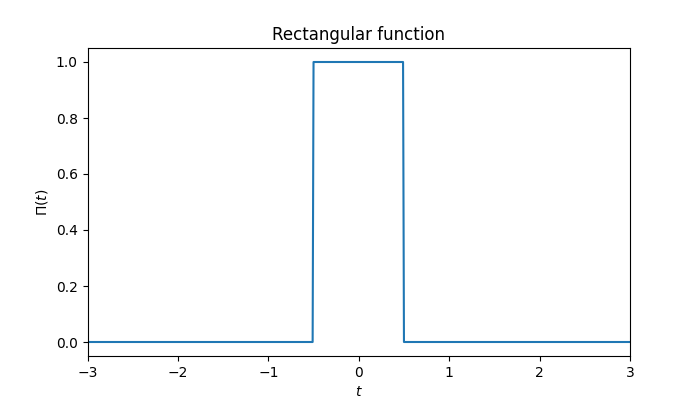
\includegraphics[width=\linewidth]{rectf.png}
            \caption{Прямоугольная функция}
            \label{fig:rectf}
        \end{subfigure}
        \hspace{5mm}
        \begin{subfigure}{0.45\textwidth}
            \centering
            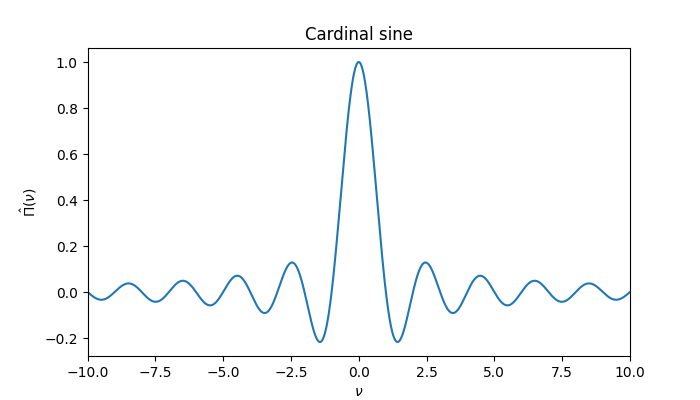
\includegraphics[width=\linewidth]{sinc.png}
            \caption{Кардинальный синус}
            \label{fig:sinc}
        \end{subfigure}
        \caption{Исходный сигнал и его Фурье-образ}
        \label{fig:rectfsinc}
    \end{figure}


    \subsection{Численное интегрирование}
    Зададим функцию $\Pi(t)$ в \texttt{Python}. Найдем ее Фурье-образ с помощью численного интегрирования (функция \texttt{trapz}).
    Вновь используя численное интегрирование, выполним обратное преобразование Фурье от найденного Фурье-образа с целью восстановить исходную функцию.
    Схематично наши действия будут выглядеть так:
    \begin{center}
        $\Pi(t)$
        \begin{tikzpicture}
            \draw[->] (0,0) -- (1,0) node[midway, above] {\tiny{\texttt{trapz}}};
        \end{tikzpicture}
        $\hat{\Pi}(\nu)$
        \begin{tikzpicture}
            \draw[->] (0,0) -- (1,0) node[midway, above] {\tiny{\texttt{trapz}}};
        \end{tikzpicture}
        $\Pi(t)$
    \end{center}
    Построим график найденной функции $\hat{\Pi}(\nu)$ и \textit{восстановленной} функции $\Pi(t)$.
    Сравним результат с истинной функцией и Фурье-образом. Исследуем влияние
    величины шага интегрирования и размера промежутка, по которому вычисляется
    интеграл, на результат. Сделаем выводы о точности и быстродействии метода.


    Далее приведены соответствующие графики. Оранжевым цветом выделены оригинальные функции, синим --
    найденные через преобразования. Каждый график подписан сверху. Под временной шкалой также указаны
    рассматриваемый промежуток времени или частот и шаг дискретизации во временной или частотной областях.
    \begin{figure}[H]
        \centering
        \begin{subfigure}{0.45\textwidth}
            \centering
            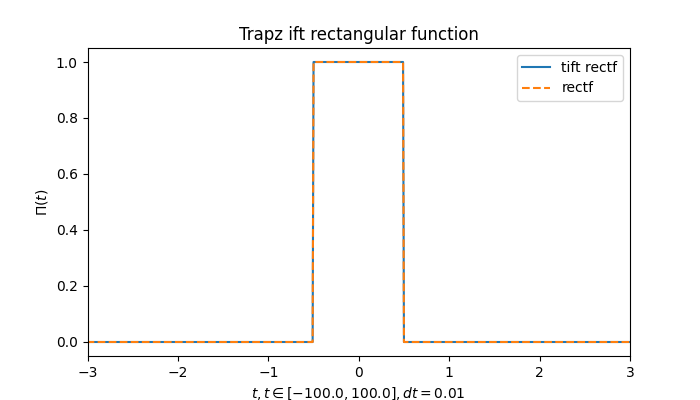
\includegraphics[width=\linewidth]{1_tiftr.png}
            \caption{$\Pi(t)$, восстановленная \texttt{trapz}}
            \label{fig:trectf1}
        \end{subfigure}
        \hspace{5mm}
        \begin{subfigure}{0.45\textwidth}
            \centering
            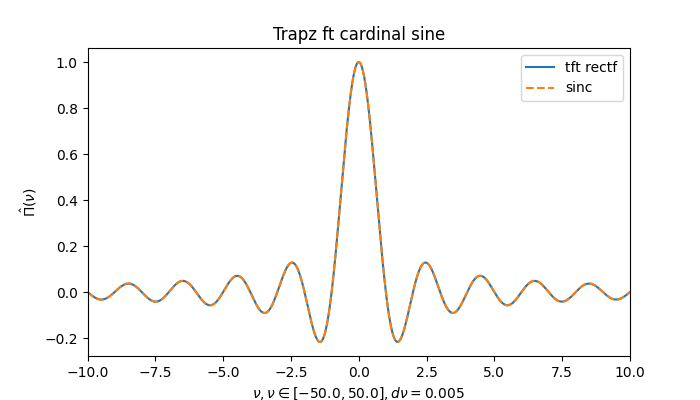
\includegraphics[width=\linewidth]{1_tftr.png}
            \caption{$\hat{\Pi}(t)$ восстановленной \texttt{trapz} $\Pi(t)$}
            \label{fig:tsinc1}
        \end{subfigure}
        \caption{Интеграл по всей области определения функции от $-100$ до $100$}
        \label{fig:trapzs1}
    \end{figure}
    \vspace{-5mm}
    \begin{figure}[H]
        \centering
        \begin{subfigure}{0.45\textwidth}
            \centering
            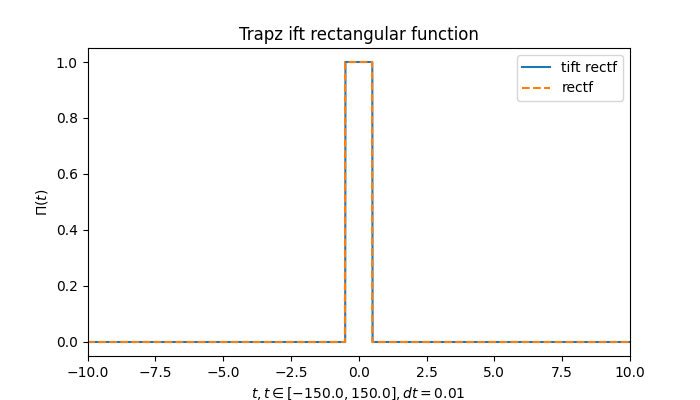
\includegraphics[width=\linewidth]{4_tiftr.png}
            \caption{$\Pi(t)$, восстановленная \texttt{trapz}}
            \label{fig:trectf4}
        \end{subfigure}
        \hspace{5mm}
        \begin{subfigure}{0.45\textwidth}
            \centering
            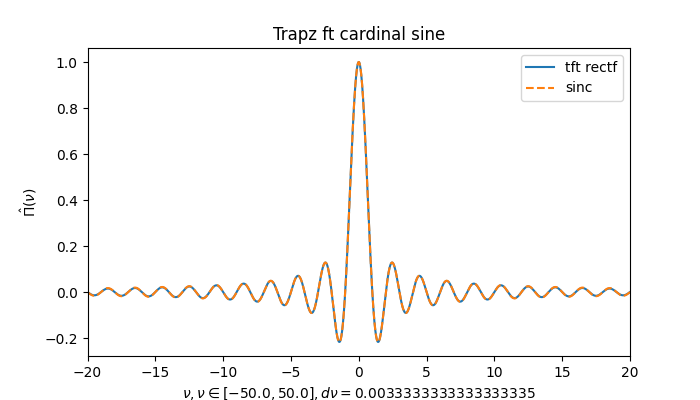
\includegraphics[width=\linewidth]{4_tftr.png}
            \caption{$\hat{\Pi}(t)$ восстановленной \texttt{trapz} $\Pi(t)$}
            \label{fig:tsinc4}
        \end{subfigure}
        \caption{Интеграл на увеличенном промежутке от $-150$ до $150$}
        \label{fig:trapzs4}
    \end{figure}
    \vspace{-5mm}
    \begin{figure}[H]
        \centering
        \begin{subfigure}{0.45\textwidth}
            \centering
            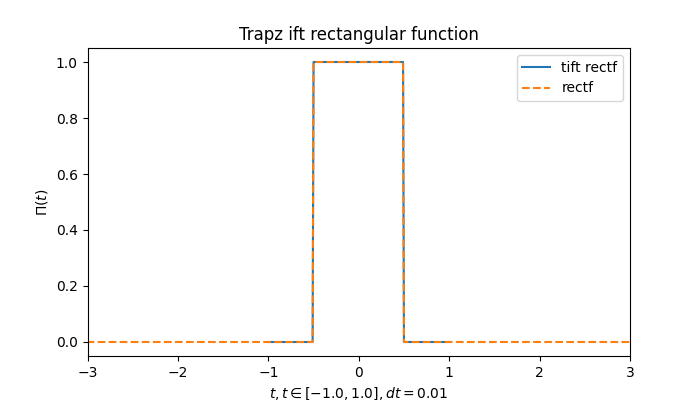
\includegraphics[width=\linewidth]{2_tiftr.png}
            \caption{$\Pi(t)$, восстановленная \texttt{trapz}}
            \label{fig:trectf2}
        \end{subfigure}
        \hspace{5mm}
        \begin{subfigure}{0.45\textwidth}
            \centering
            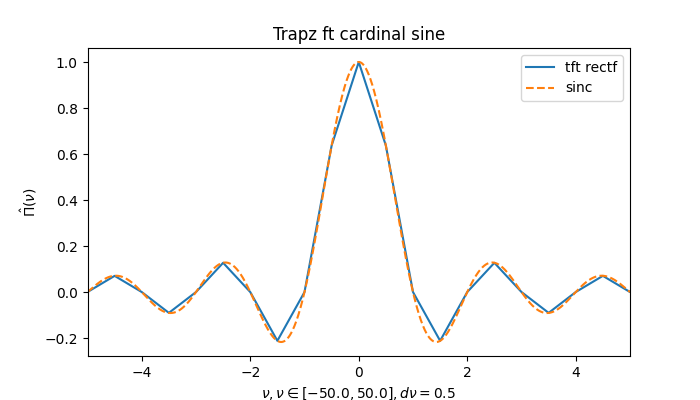
\includegraphics[width=\linewidth]{2_tftr.png}
            \caption{$\hat{\Pi}(t)$ восстановленной \texttt{trapz} $\Pi(t)$}
            \label{fig:tsinc2}
        \end{subfigure}
        \caption{Интеграл на уменьшенном промежутке от $-1$ до $1$}
        \label{fig:trapzs2}
    \end{figure}
    \vspace{-5mm}
    \begin{figure}[H]
        \centering
        \begin{subfigure}{0.45\textwidth}
            \centering
            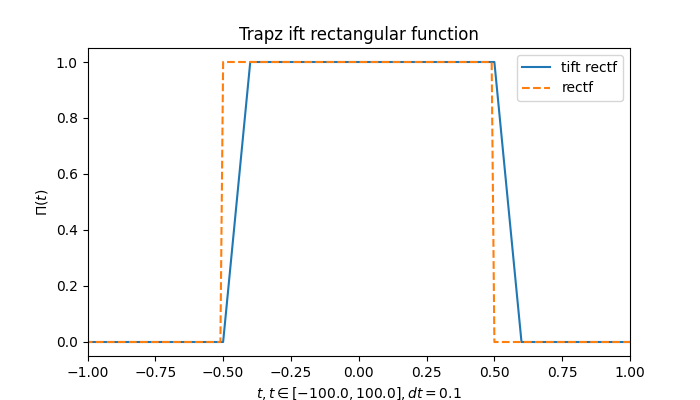
\includegraphics[width=\linewidth]{3_tiftr.png}
            \caption{$\Pi(t)$, восстановленная \texttt{trapz}}
            \label{fig:trectf3}
        \end{subfigure}
        \hspace{5mm}
        \begin{subfigure}{0.45\textwidth}
            \centering
            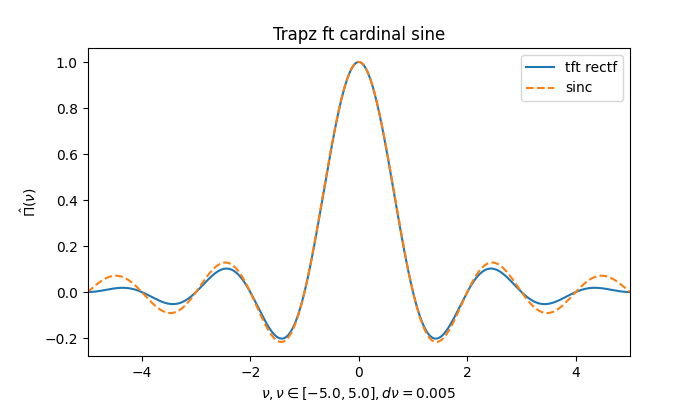
\includegraphics[width=\linewidth]{3_tftr.png}
            \caption{$\hat{\Pi}(t)$ восстановленной \texttt{trapz} $\Pi(t)$}
            \label{fig:tsinc3}
        \end{subfigure}
        \caption{Увеличение шага интегрирования $dt=0.1$, интеграл аналогично рис. \ref{fig:trapzs1}}
        \label{fig:trapzs3}
    \end{figure}
    \begin{figure}[H]
        \centering
        \begin{subfigure}{0.45\textwidth}
            \centering
            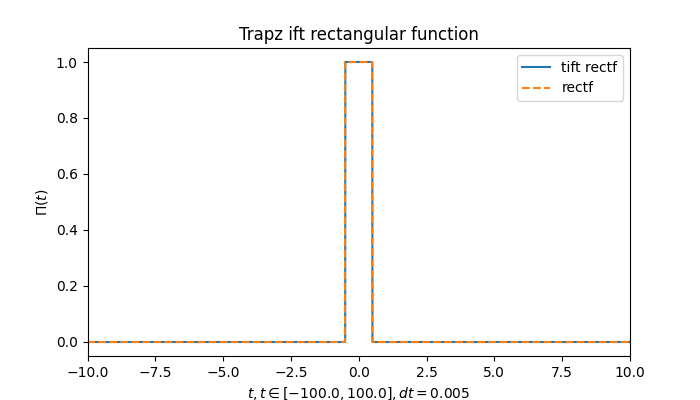
\includegraphics[width=\linewidth]{5_tiftr.png}
            \caption{$\Pi(t)$, восстановленная \texttt{trapz}}
            \label{fig:trectf5}
        \end{subfigure}
        \hspace{5mm}
        \begin{subfigure}{0.45\textwidth}
            \centering
            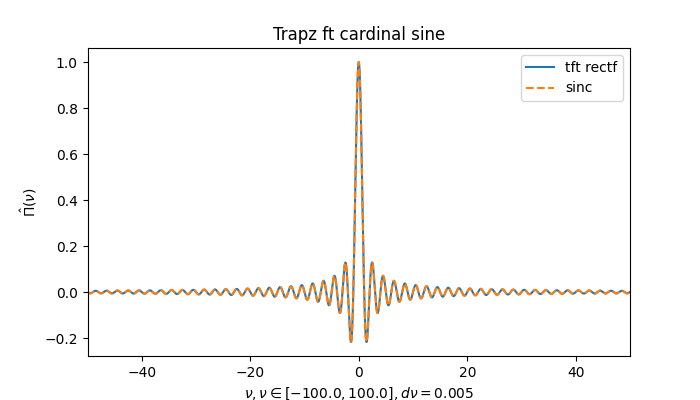
\includegraphics[width=\linewidth]{5_tftr.png}
            \caption{$\hat{\Pi}(t)$ восстановленной \texttt{trapz} $\Pi(t)$}
            \label{fig:tsinc5}
        \end{subfigure}
        \caption{Уменьшение шага интегрирования $dt=0.005$, интеграл аналогично рис. \ref{fig:trapzs1}}
        \label{fig:trapzs5}
    \end{figure}


    Исходя из графиков можно сделать вывод, что \texttt{trapz} имеет высокую точность аппроксимации исходного сигнала и
    его Фурье-образа, однако ее мы достигаем при маленьком шаге $dt$ и большом промежутке $T$ (см. рис. \ref{fig:trapzs1}, \ref{fig:trapzs4}, \ref{fig:trapzs5}),
    что увеличивает вычислительную сложность метода. В итоге приходится долго ждать получения результата. При уменьшении
    промежутка интегрирования \texttt{trapz} выдает точный результат прямоугольной функции (см. рис. \ref{fig:trapzs2}),
    однако Фурье-образ становится негладким. При большом шаге интегрирования подсчеты происходят быстро, но
    теряется точность функций во временной и частотных областях (см. рис. \ref{fig:trapzs3}). Таким образом, метод точный,
    но затрачивает много времени на вычисления.


    \subsection{Использование DFT}
    Найдем Фурье-образ функции $\Pi(t)$ с помощью дискретного преобразования Фурье (конструкция \texttt{fftshift(fft())}), используя его так,
    чтобы преобразование было унитарным. Выполним обратное преобразование от
    найденного Фурье-образа с помощью обратного дискретного преобразования (конструкция \texttt{ifft(ifftshift())}). Схематично наши действия можно представить так:
    \begin{center}
        $\Pi(t)$
        \begin{tikzpicture}
            \draw[->] (0,0) -- (2,0) node[midway, above] {\tiny{\texttt{fftshift(fft())}}};
        \end{tikzpicture}
        $\hat{\Pi}(\nu)$
        \begin{tikzpicture}
            \draw[->] (0,0) -- (2,0) node[midway, above] {\tiny{\texttt{ifft(ifftshift())}}};
        \end{tikzpicture}
        $\Pi(t)$
    \end{center}


    Для того, чтобы преобразование было унитарным, необходимо домножить ряд дискретного преобразования Фурье
    на коэффициент $$\dfrac{1}{\sqrt{N}},\ \ N \text{ -- количество членов ряда.}$$ Аналогично для обратного преобразования Фурье. Таким образом, формулы DFT и IDFT будут
    иметь вид:
    $$
    \mathcal{F}_m = \dfrac{1}{\sqrt{N}}\sum\limits_{n=0}^{N-1}f_ne^{-2\pi i \frac{mn}{N}},\ \ f_n=\dfrac{1}{\sqrt{N}}\sum\limits_{m=0}^{N-1}\mathcal{F}_me^{2\pi i\frac{mn}{N}}
    $$
    Далее приведены сравнительные графики найденной $\hat{\Pi}(\nu)$ и \textit{восстановленной} $\Pi(t)$ функций с исходными. Цвета и обозначения аналогичны предыдущему пункту.


    Исходя из графиков можно сделать вывод, что унитарное быстрое преобразование Фурье точно восстанавливает
    исходный сигнал, затрачивая малое количество времени на вычисления. Однако Фурье-образ не совпадает с истинным (кардинальным синусом).
    Функция приобрела лишние амплитуды на всей частотной области  (см. рис. \ref{fig:uffts}).
    \begin{figure}[H]
        \centering
        \begin{subfigure}{0.45\textwidth}
            \centering
            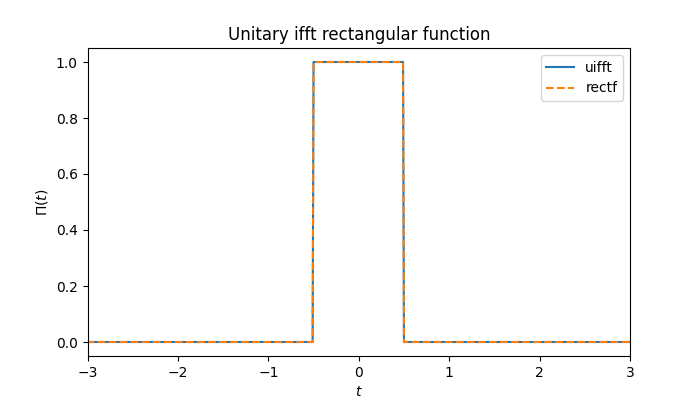
\includegraphics[width=\linewidth]{uifft.png}
            \caption{$\Pi(t)$, восстановленная \texttt{ufft}}
            \label{fig:uifft}
        \end{subfigure}
        \hspace{5mm}
        \begin{subfigure}{0.45\textwidth}
            \centering
            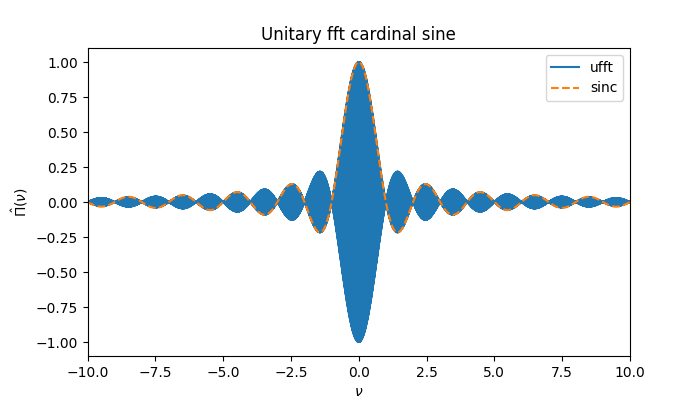
\includegraphics[width=\linewidth]{ufft.png}
            \caption{$\hat{\Pi}(t)$ восстановленной \texttt{ufft} $\Pi(t)$}
            \label{fig:ufft}
        \end{subfigure}
        \begin{subfigure}{0.45\textwidth}
            \centering
            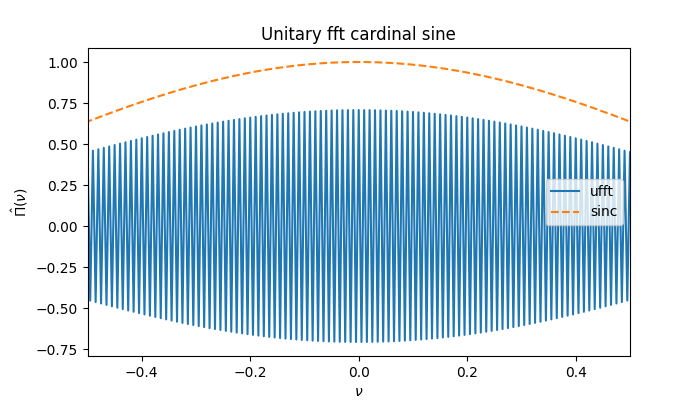
\includegraphics[width=\linewidth]{ufft_close.png}
            \caption{Рис. (b) в приближении}
            \label{fig:ufftc}
        \end{subfigure}
        \caption{Унитарное быстрое преобразование Фурье \texttt{ufft}}
        \label{fig:uffts}
    \end{figure}


    \subsection{Выводы о trapz и fft}
    Метод \texttt{trapz} работает медленно, но точно -- он смог приблизиться к истинному Фурье-образу прямоугольной функции.
    \texttt{trapz} выполняет численное интегрирование с помощью трапециевидного метода -- он аппроксимирует интегрирование
    на интервале путем разламывания области на трапецоиды с более легко вычислимыми областями. Для интеграции с $N+1$
    равномерно распределенными точками приближение будет иметь вид:
    $$
    \int\limits_{a}^{b}f(x)\,dx\approx\dfrac{b-a}{2N}\sum\limits_{n=1}^{N}\left(f(x_n)+f(x_{n+1})\right), \ \ \dfrac{b-a}{N} \text{ -- интервал между каждой точкой.}
    $$
    К выражению выше добавляется умножение на экспоненту, в степени которой находится переменная, по которой вычисляется интеграл.
    Обратное преобразование находится аналогично.


    Метод \texttt{fft} работает быстро, но Фурье-образ не похож на кардинальный синус. В предыдущем пункте были приведены
    формулы, которые используются для дискретного преобразования Фурье -- через них работает быстрое преобразование Фурье.
    \texttt{fft} основывается на <<симметриях>> корней из единицы матрицы \texttt{dft}, которую можно составить из элементов
    одноименного ряда. Эта матрица квадратная и обратимая, иначе мы не смогли бы найти \texttt{idft}. Более того, она
    унитарная -- обратная матрица является транспонированной комплексно-сопряженной -- воздействует как <<поворот>>.
    Симметрия корней из 1 связана с тем, что значения $\omega_{N}^k=e^{2\pi i k\div N}$ делятся на две группы:
    те, у которых $k$ четное, и те, у которых $k$ нечетное. При этом $\omega_{N}^{N\div2}$ является корнем из -1.


    Фурье-образ получается лучше у метода трапеций, так как он проходит по каждому значению времени и вычисляет
    в приближении сложный интеграл. Однако у \texttt{fft} по времени лучше получается восстановленный сигнал несмотря на то,
    что Фурье-образ не совпадает с истинным. Причина в тех симметриях, о которых написано в абзаце выше -- алгоритмы
    \texttt{fft} и \texttt{ifft} взаимно обратны. Ошибки округления и другие численные погрешности, возникающие при прямом преобразовании,
    компенсируются при обратном преобразовании.


    \subsection{Приближение непрерывного с помощью DFT}
    Чтобы исправить ситуацию, попробуем совместить достоинства обоих подходов: точность и быстродействие.
    Найдем способ получить правильный Фурье-образ, соответствующий непрерывному преобразованию Фурье, используя функцию \texttt{fft} и не прибегая к численному
    интегрированию. Найдем способ восстановить исходный сигнал по полученному
    Фурье-образу -- тоже с помощью \texttt{fft}. Схема нашего успеха:
    \begin{center}
        $\Pi(t)$
        \begin{tikzpicture}
            \draw[->] (0,0) -- (3,0) node[midway, above] {\tiny{умное использование \texttt{fft}}};
        \end{tikzpicture}
        $\hat{\Pi}(\nu)$
        \begin{tikzpicture}
            \draw[->] (0,0) -- (3,0) node[midway, above] {\tiny{умное использование \texttt{ifft}}};
        \end{tikzpicture}
        $\Pi(t)$
    \end{center}


    Ранее мы выяснили, что метод трапеций работает наиболее точно, но он ресурсозатратен.
    \begin{figure}[H]
        \centering
        \begin{subfigure}{0.45\textwidth}
            \centering
            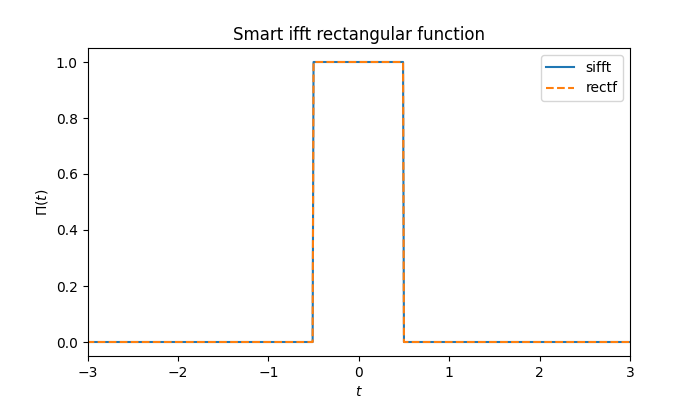
\includegraphics[width=\linewidth]{sifft.png}
            \caption{$\Pi(t)$, восстановленная \texttt{sfft}}
            \label{fig:sifft}
        \end{subfigure}
        \hspace{5mm}
        \begin{subfigure}{0.45\textwidth}
            \centering
            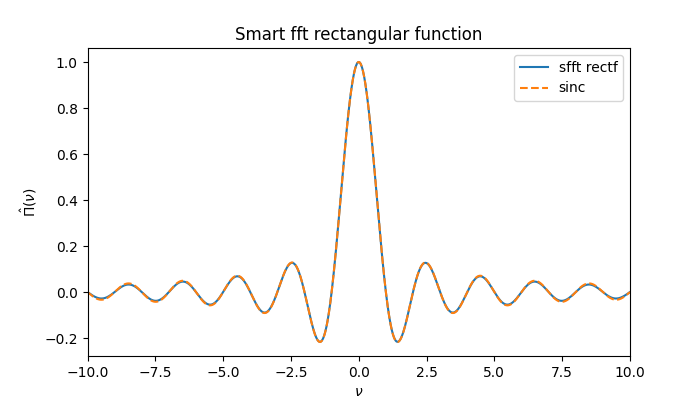
\includegraphics[width=\linewidth]{sfft.png}
            \caption{$\hat{\Pi}(t)$ восстановленной \texttt{sfft} $\Pi(t)$}
            \label{fig:sfft}
        \end{subfigure}
        \caption{Умное использование быстрого преобразования Фурье \texttt{sfft}}
        \label{fig:sffts}
    \end{figure}


    \section{Задание 2. Сэмплирование}
    В этом задании будем исследовать теорему Найквиста-Шеннона-Котельникова на двух примерах.
    \subsection{Сэмплирование синусов}
    Зададим параметры $a_1=1,\,a_2=2,\,\omega_1=3,\,\omega_2=4,\,\varphi_1=\pi\div5,\,\varphi_2=\pi\div6$ и рассмотрим функцию
    $$y(t)=a_1\sin{(\omega_1t+\varphi_1)}+a_2\sin{(\omega_2t+\varphi_2)}$$


    Зададим в \texttt{Python} массивы времени \texttt{t} и значений \texttt{y}. Выберем малый шаг дискретизации $dt=10^{-4}$ для
    имитирования непрерывной функции. Построим график полученной функции.
    \begin{figure}[H]
        \centering
        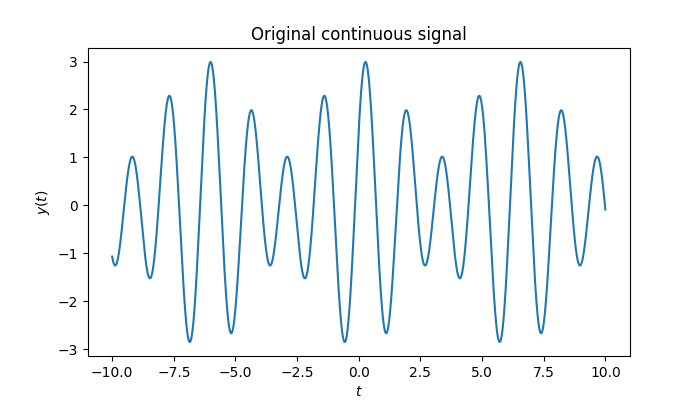
\includegraphics[scale=0.45]{orig1.png}
        \captionsetup{skip=0pt}
        \caption{График непрерывного сигнала}
        \label{fig:orig1}
    \end{figure}


    Теперь зададим сэмплированный вариант указанной функции: рассмотрим
    разреженный вариант массива времени и соответствующий ему массив значений.
    Сначала рассмотрим большой шаг $dt=0.2$.
    Построим дискретный график поверх непрерывного.
    \begin{figure}[H]
        \centering
        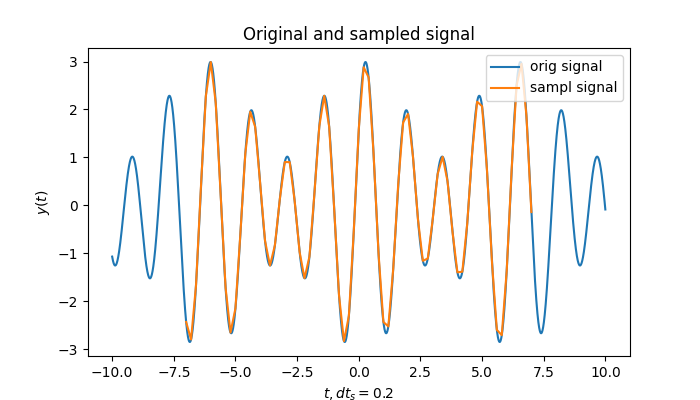
\includegraphics[scale=0.45]{1_sine.png}
        \captionsetup{skip=0pt}
        \caption{График сэмплированного сигнала поверх непрерывного}
        \label{fig:1sine}
    \end{figure}


    Применим интерполяционную формулу из лекции к сэмплированным
    данным с целью восстановить непрерывную функцию.
    $$
    f(t)=\sum\limits_{n=-\infty}^{\infty}f(t_n)\cdot\sinc{(2B(t-t_n))},\ \ t_n=\dfrac{n}{2B}
    $$
    В результате получатся новые массивы времени и значений -- той же размерности, что и исходные.


    Построим график восстановленной функции поверх исходной.
    \begin{figure}[H]
        \centering
        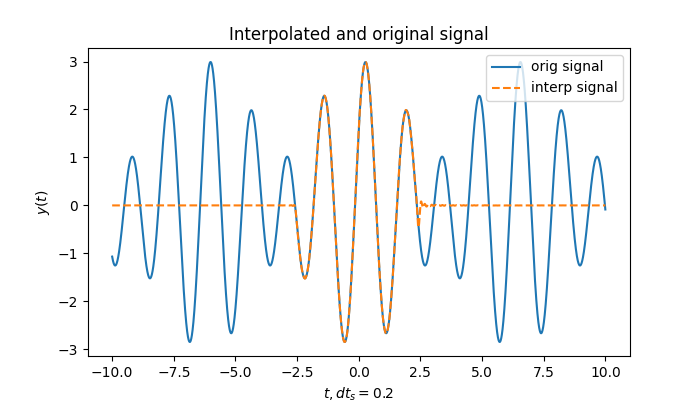
\includegraphics[scale=0.45]{1_isine.png}
        \captionsetup{skip=0pt}
        \caption{График интерполированного сигнала поверх непрерывного}
        \label{fig:1isine}
    \end{figure}
    

    Далее исследуем влияние шага дискретизации на вид восстановленной функции
    и соотнесем свои результаты с теоремой Найквиста-Шеннона-Котельникова. Синим цветом выделены исходные сигналы, оранжевым --
    сэмплированные и восстановленные. Под шкалой времени на каждом графике указан шаг дискретизации сэмплирования $dt_s$.
    \begin{figure}[H]
        \centering
        \begin{subfigure}{0.45\textwidth}
            \centering
            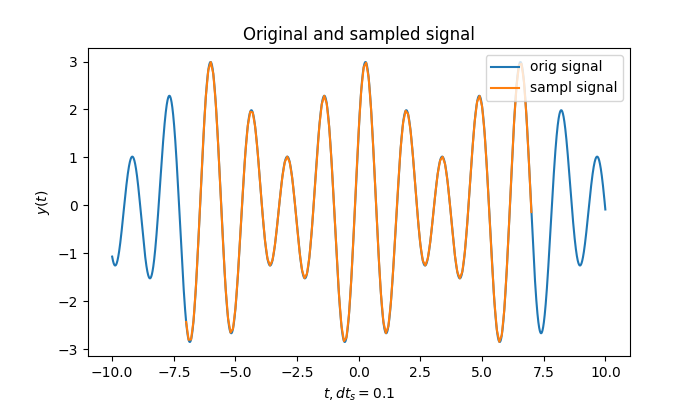
\includegraphics[width=\linewidth]{2_sine.png}
            \caption{Cэмплированный поверх непрерывного}
            \label{fig:2sine}
        \end{subfigure}
        \hspace{5mm}
        \begin{subfigure}{0.45\textwidth}
            \centering
            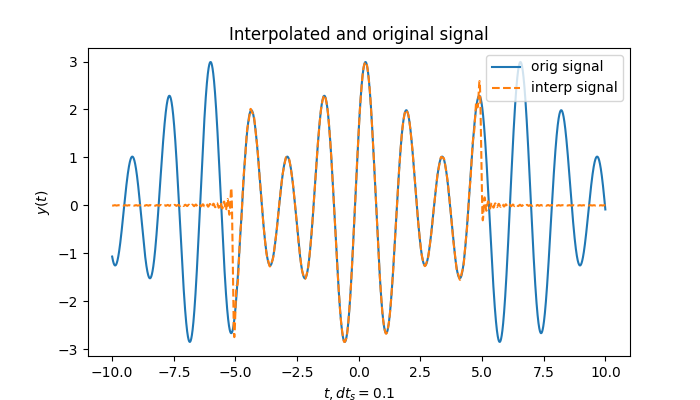
\includegraphics[width=\linewidth]{2_isine.png}
            \caption{Интерполированный поверх непр-ого}
            \label{fig:2isine}
        \end{subfigure}
        \caption{Уменьшение шага дискретизации $dt=0.1$}
        \label{fig:sines2}
    \end{figure}
    \begin{figure}[H]
        \centering
        \begin{subfigure}{0.45\textwidth}
            \centering
            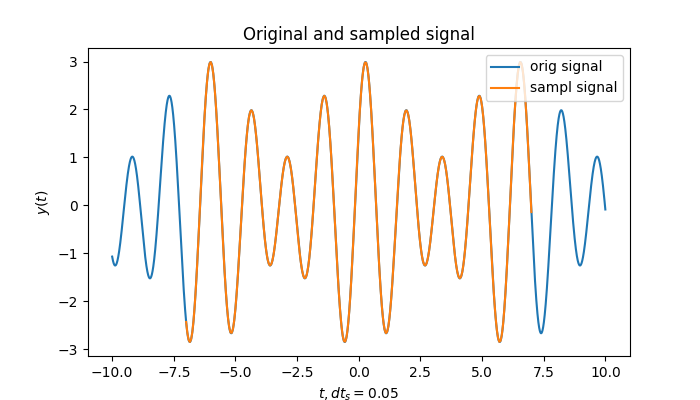
\includegraphics[width=\linewidth]{3_sine.png}
            \caption{Cэмплированный поверх непр-ого}
            \label{fig:3sine}
        \end{subfigure}
        \hspace{5mm}
        \begin{subfigure}{0.45\textwidth}
            \centering
            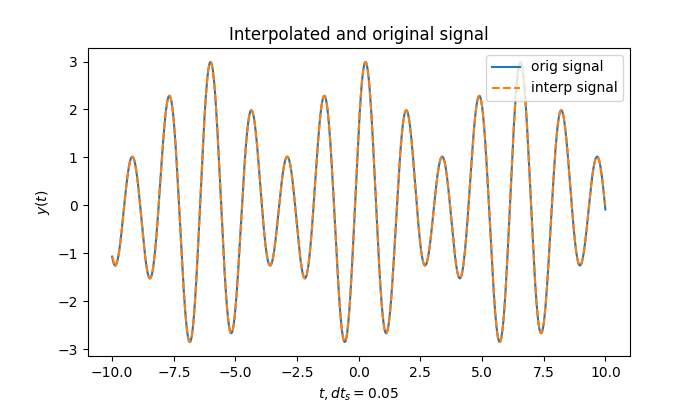
\includegraphics[width=\linewidth]{3_isine.png}
            \caption{Интерполированный поверх непр-ого}
            \label{fig:3isine}
        \end{subfigure}
        \caption{Уменьшение шага дискретизации $dt=0.05$}
        \label{fig:sines3}
    \end{figure}


    \subsection{Сэмплирование sinus cardinalis}
    Зададим параметр $b=2$ и рассмотрим функцию $$y(t)=\sinc{(bt)}=\sinc{(2t)}$$
    Выполним все шаги из предыдущего пункта. Дополнительно для каждой величины
    шага дискретизации построим Фурье-образ исходного и
    восстановленного сигналов. Дадим объяснение увиденному, сделаем выводы.
    \begin{figure}[H]
        \centering
        \begin{subfigure}{0.45\textwidth}
            \centering
            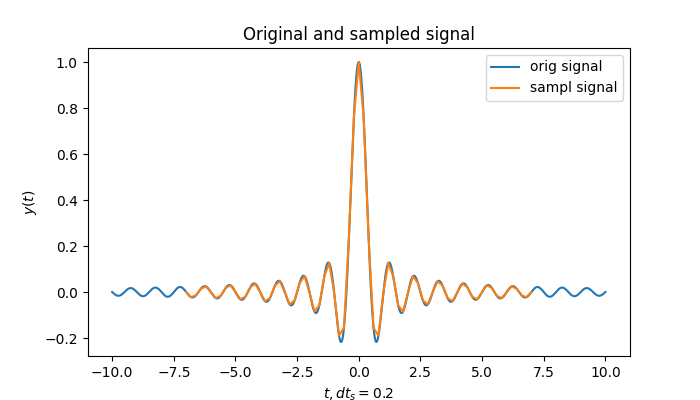
\includegraphics[width=\linewidth]{1_sinc.png}
            \caption{Cэмплированный поверх непр-ого}
            \label{fig:sinc1}
        \end{subfigure}
        \hspace{5mm}
        \begin{subfigure}{0.45\textwidth}
            \centering
            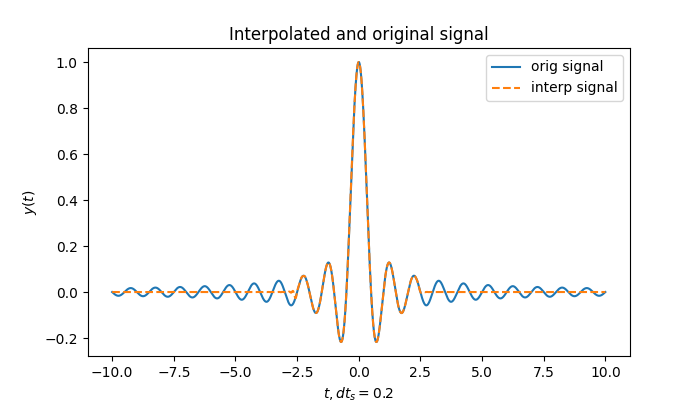
\includegraphics[width=\linewidth]{1_isinc.png}
            \caption{Интерполированный поверх непр-ого}
            \label{fig:isinc1}
        \end{subfigure}
        \begin{subfigure}{0.45\textwidth}
            \centering
            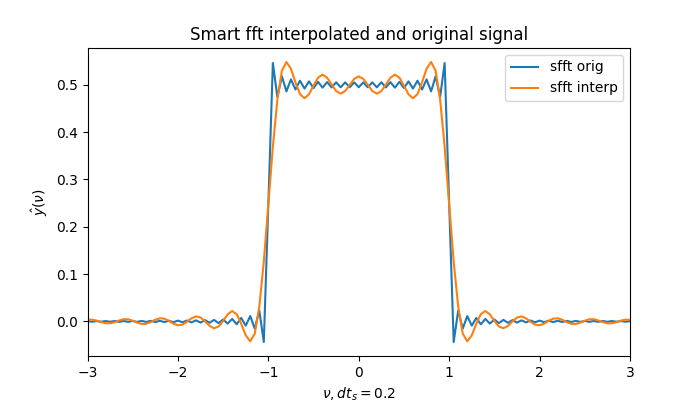
\includegraphics[width=\linewidth]{1_fsinc.png}
            \caption{Фурье-образ}
            \label{fig:fisinc1}
        \end{subfigure}
        \caption{Подпись}
        \label{fig:sincs1}
    \end{figure}
    \begin{figure}[H]
        \centering
        \begin{subfigure}{0.45\textwidth}
            \centering
            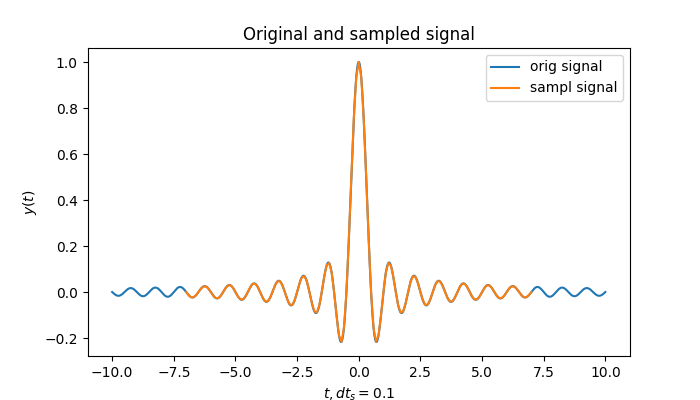
\includegraphics[width=\linewidth]{2_sinc.png}
            \caption{Cэмплированный поверх непр-ого}
            \label{fig:sinc2}
        \end{subfigure}
        \hspace{5mm}
        \begin{subfigure}{0.45\textwidth}
            \centering
            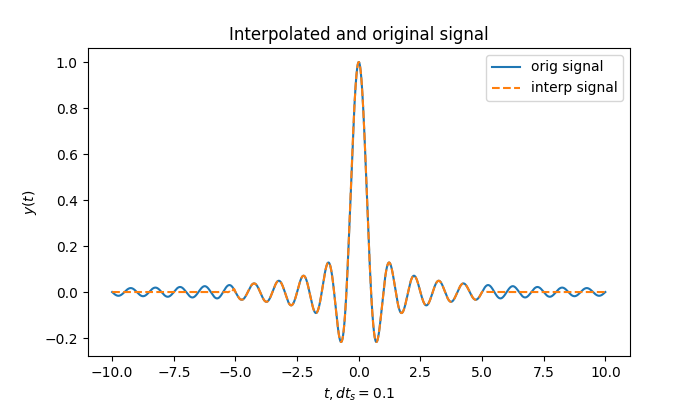
\includegraphics[width=\linewidth]{2_isinc.png}
            \caption{Интерполированный поверх непр-ого}
            \label{fig:isinc2}
        \end{subfigure}
        \begin{subfigure}{0.45\textwidth}
            \centering
            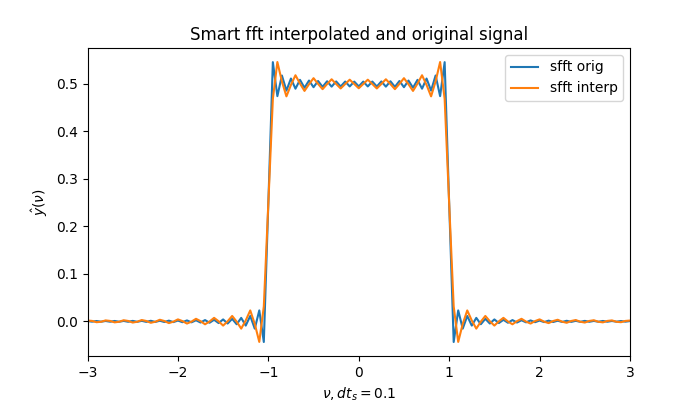
\includegraphics[width=\linewidth]{2_fsinc.png}
            \caption{Фурье-образ}
            \label{fig:fisinc2}
        \end{subfigure}
        \caption{Подпись}
        \label{fig:sincs2}
    \end{figure}
    \begin{figure}[H]
        \centering
        \begin{subfigure}{0.45\textwidth}
            \centering
            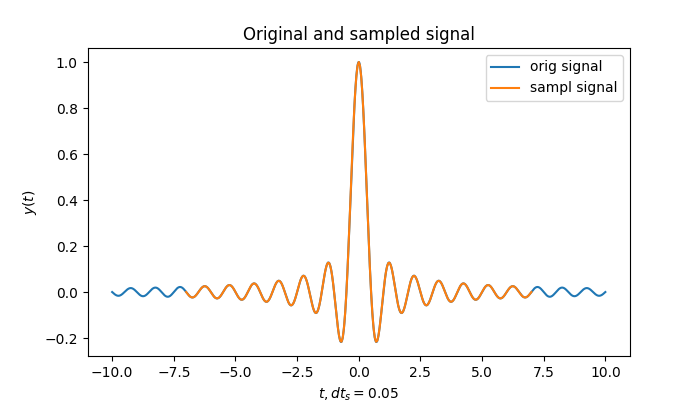
\includegraphics[width=\linewidth]{3_sinc.png}
            \caption{Cэмплированный поверх непр-ого}
            \label{fig:sinc3}
        \end{subfigure}
        \hspace{5mm}
        \begin{subfigure}{0.45\textwidth}
            \centering
            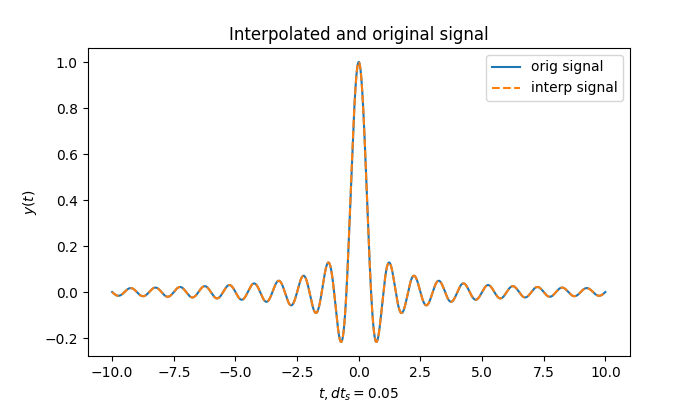
\includegraphics[width=\linewidth]{3_isinc.png}
            \caption{Интерполированный поверх непр-ого}
            \label{fig:isinc3}
        \end{subfigure}
        \begin{subfigure}{0.45\textwidth}
            \centering
            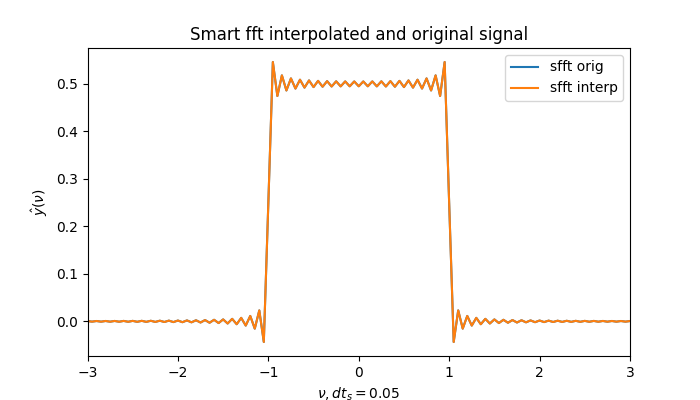
\includegraphics[width=\linewidth]{3_fsinc.png}
            \caption{Фурье-образ}
            \label{fig:fisinc3}
        \end{subfigure}
        \caption{Подпись}
        \label{fig:sincs3}
    \end{figure}
\end{document}